% Copyright 2020 by Robert Hildebrand
%This work is licensed under a
%Creative Commons Attribution-ShareAlike 4.0 International License (CC BY-SA 4.0)
%See http://creativecommons.org/licenses/by-sa/4.0/% 



\documentclass[../open-optimization/open-optimization.tex]{subfiles}
 
\begin{document}

\chapter{Integer Programming Formulations}
\label{sec:IP-formulations} 
\section{Knapsack Problem}
Knapsack problem can take different forms depending on if the variables are binary or integer.  The binary version means that there is only one item of each item type that can be taken.  This is typically illustrated as a backpack (knapsack) and some items to put into it (see  \autoref{fig:wiki/File/knapsack}), but has applications in many contexts.  

 \includefigurestatic[Knapsack Problem: which items should we choose take in the knapsack that maximizes the value while respecting the 15kg weight limit?][width=.4\linewidth][h]{wiki/File/knapsack}

\begin{general}{Binary Knapsack Problem}{\npcomplete}
Given an non-negative weight vector $a \in \Q^n_+$, a capacity $b \in \Q_+$, and objective coefficients $c \in \Q^n$, 
\begin{equation}
\begin{split}
\max \ \ & c^\top x\\
\text{s.t.}\ \ & a^\top x \leq b\\
& x \in \{0,1\}^n
\end{split}
\end{equation}
\end{general}
 


 
%\begin{figure}[H]
%\begin{center}
%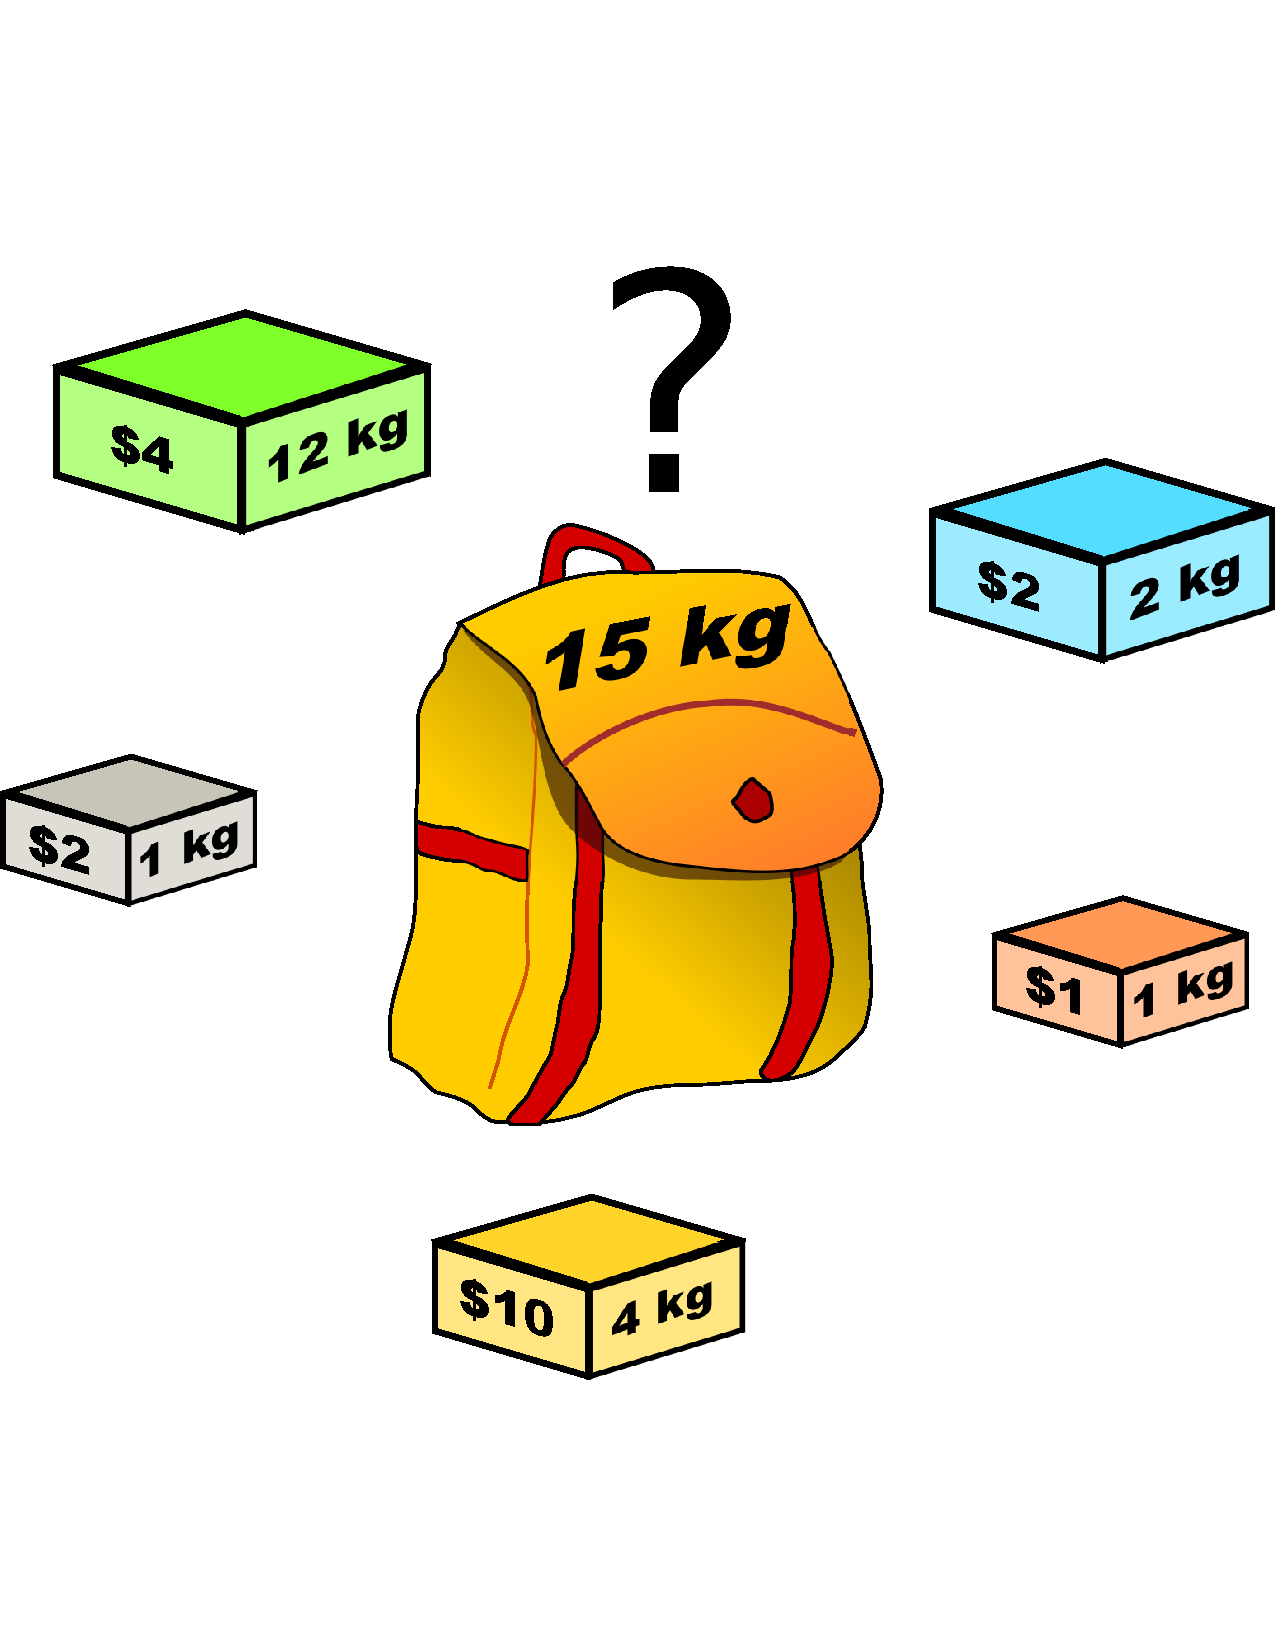
\includegraphics[scale = 0.2]{knapsack}\footnotemark 
%\end{center}
%\label{fig:knapsack}
%\caption{Knapsack Problem: which items should we choose take in the knapsack that maximizes the value while respecting the 15kg weight limit?}
%\end{figure}
%\footnotetext{\url{https://en.wikipedia.org/wiki/Knapsack_problem}}

\begin{examplewithcode}{Knapsack}{code:knapsack}
\label{example:knapsack}
You have a knapsack (bag) that can only hold W = 15 kgs.  There are 5 items that you could possibly put into your knapsack.  The items (weight, value) are given as:
(12 kg, $\$$4), (2 kg, $\$$2), (1kg, $\$$2), (1kg, $\$$1), (4kg, $\$$10).  Which items should you take to maximize your value in the knapsack? See \autoref{fig:wiki/File/knapsack}.\\

\noindent \textbf{Variables:}
\begin{itemize}
\item let $x_i = 0$ if item $i$ is in the bag
\item let $x_i = 1$ if item $i$ is not in the bag
\end{itemize}
\textbf{Model:}
\begin{equation}
\begin{split}
\max  \  \ &4 x_1 + 2 x_2 + 2 x_3 + 1 x_4 + 10 x_5\\
\text{ s.t. }\ \ &  12 x_1 + 2 x_2 + 1 x_3 + 1 x_4 + 4 x_5 \leq 15\\
& x_i \in \{0,1\} \text{ for } i=1, \dots, 5
\end{split}
\end{equation}
\end{examplewithcode}
In the integer case, we typically require the variables to be non-negative integers, hence we use the notation $x \in \Z^n_+$.  This setting reflects the fact that instead of single individual items, you have item types of which you can take as many of each type as you like that meets the constraint.
\begin{general}{Integer Knapsack Problem}{\npcomplete}
Given an non-negative weight vector $a \in \Q^n_+$, a capacity $b \in \Q_+$, and objective coefficients $c \in \Q^n$, 
\begin{equation}
\begin{split}
\max \ \ & c^\top x\\
\text{s.t.}\ \ & a^\top x \leq b\\
& x \in \Z^n_+
\end{split}
\end{equation}
\end{general}
We can also consider an equality constrained version
\begin{general}{Equality Constrained Integer Knapsack Problem}{\nphard}
Given an non-negative weight vector $a \in \Q^n_+$, a capacity $b \in \Q_+$, and objective coefficients $c \in \Q^n$, 
\begin{align}
\max \ \ & c^\top x\\
\text{s.t.}\ \ & a^\top x = b\\
& x \in \Z^n_+
\end{align}
\end{general}
\begin{example}
\label{ex:min-coins}
Using pennies, nickels, dimes, and quarters, how can you minimize the number of coins you need to to make up a sum of $83\cent$? 

\textbf{Variables:}
\begin{itemize}
\item Let $p$ be the number of pennies used
\item Let $n$ be the number of nickels used
\item Let $d$ be the number of dimes used
\item Let $q$ be the number of quarters used
\end{itemize}
\textbf{Model}
\begin{align*}
\min \quad & p + n + d + q & \text{ total number of coins used}\\
\text{ s.t. } \quad & p + 5n + 10d + 25 q = 83 & \text{sums to } 83 \cent\\
& p,d,n,q \in \Z_+ & \text{each is a non-negative integer}
\end{align*}
\end{example}
\section{Set Covering}
\begin{general}{Set Covering}{\npcomplete}
\label{general:set-covering}
Given a set $V$ with subsets $V_1, \dots, V_l$, determine the smallest subset $S \subseteq V$ such that 
$S \cap V_i \neq \emptyset$ for all $i=1, \dots, l$.

The set cover problem can be modeled as
\begin{equation}
\begin{split}
\min \ \ & \one^\top x\\
\text{s.t.} \ \ & \sum_{v \in V_i} x_v \geq 1 \text{ for all } i =1, \dots, l \\ 
& x_v \in \{0,1\} \text{ for all } v \in V
\end{split}
\end{equation}
where $x_v$ is a 0/1 variable that takes the value $1$ if we include item $j$ in set $S$ and $0$ if we do not include it in the set $S$.  
\end{general}

\begin{todo}
Add flight crew scheduling example and images.
\end{todo}

One specific type of set cover problem is the \emph{vertex cover} problem.
\begin{general}{Vertex Cover}{\npcomplete}
Given a graph $G = (V,E)$ of vertices and edges, we want to find a smallest size subset $S \subseteq V$ such that every for every $e = (v,u) \in E$, either $u$ or $v$ is in $S$.   

We can write this as a mathematical program in the form:
\begin{equation}
\begin{split}
\min \ \ & \one^\top x\\
\text{s.t.} \ \ & x_u + x_v \geq 1 \text{ for all } (u,v) \in E \\ 
& x_v \in \{0,1\} \text{ for all } v \in V.
\end{split}
\end{equation}
\end{general}

\begin{todo}
Add fire station cover example.
\end{todo}




%\documentclass[../open-optimization/open-optimization.tex]{subfiles}

%%%%%%%%%
%\begin{document}
%%%%%%%%%

\begin{general}{Set Covering - Matrix description}{\npcomplete}
\label{general:set-covering-alternate}
Given a non-negative matrix $A \in \{0,1\}^{m \times n}$, a non-negative vector, and an objective vector $c \in \R^n$, the set cover problem is
\begin{equation}
\begin{split}
\max \ \ & c^\top x\\
\text{s.t.}. \ \ & Ax \geq \one \\
& x \in \{0,1\}^n.
\end{split}
\end{equation}
\end{general}
\begin{examplewithoutcode}{Vertex Cover with matrix}{code:vertex-cover-matrix}
An alternate way to solve \nameref{ex:vertex-cover} is to define the \emph{adjacency matrix} $A$ of the graph.  The adjacency matrix is a $|E| \times |V|$ matrix with $\{0,1\}$ entries.  The each row corresponds to an edge $e$ and each column corresponds to a node $v$.  For an edge $e = (u,v)$, the corresponding row has a $1$ in columns corresponding to the nodes $u$ and $v$, and a 0 everywhere else.  Hence, there are exactly two 1's per row.  Applying the formulation above in \nameref{general:set-covering-alternate} models the problem.
\end{examplewithoutcode}




%%%%%%%%%
%\end{document}
%%%%%%%%%




\subsubsection{General Set Covering}
We could also allow for a more general type of set covering where we have non-negative integer variables and a right hand side that has values other than $1$.
\begin{general}{Set Covering - Generalized}{\npcomplete}
\label{general:set-covering-alternate}
Given a non-negative matrix $A \in \Z_+^{m \times n}$, a non-negative vector $b \in \Z^m$, and an objective vector $c \in \R^n$, the set cover problem is
\begin{equation}
\begin{split}
\max \ \ & c^\top x\\
\text{s.t.}. \ \ & Ax \geq b \\
& x \in\Z^n_+.
\end{split}
\end{equation}
\end{general}

\begin{todo}
 Add Nurse scheduling problem.
\end{todo}

\begin{examplewithcode}{Nurse Scheduling}{code:nurse-scheduling}

\end{examplewithcode}

\section{Machine Assignment}


Example Model: Machine assignment\\

\begin{minipage}{0.6\textwidth}
\begin{itemize}
	\item Given $m$ machines and $n$ jobs, find a least cost assignment
	of jobs to machines not exceeding the machine capacities.
	\item Each job $j$ requires $a_{ij}$ units of machine $i$'s capacity $b_i$.
	\item Cost of assigning job $j$ to machine $i$ is $c_{ij}$.
	\end{itemize}
\end{minipage}
\begin{minipage}{0.3\textwidth}
\begin{todo}
Include picture
\end{todo}
%\includegraphics[scale = 0.5]{assignment}
\end{minipage}


Here is a model....  \textbf{To be added....}

\section{Facility Location}

\begin{todo}
Add discussion on Facility Location Problems and pictures.
\end{todo}
\href{https://en.wikipedia.org/wiki/Facility_location_problem}{Wikipedia - Facility Location Problem}



\subsection{Capacitated Facility Location}

\begin{general}{Capacitated Facility Location}{\npcomplete}
Given costs connections $c_{ij}$ and fixed building costs $f_i$, demands $d_j$ and capacities $u_i$, the capacitated facility location problem is 
\begin{equation}
\begin{array}{rl}
\min & \displaystyle\sum_{i=1}^n\sum_{j=1}^mc_{ij}y_{ij}+\sum_{i=1}^nf_ix_i \\
\text{s.t.} & \displaystyle\sum_{i=1}^ny_{ij}=1 \text{ for all }j=1,\dots,m \\
& \displaystyle \sum_{j=1}^md_jy_{ij}\leqslant u_ix_i\text{ for all }i=1\dots,n \\
&y_{ij}\geqslant0\text{ for all }i=1,\dots,n \text{ and }j=1,\dots,m\\
&x_i\in\{0,1\}\text{ for all } i=1,\dots,n
\end{array}
\end{equation}
Here $M$ is a large number and can be chosen as $M = m$, but could be refined smaller if more context is known.
\end{general}

\subsection{Uncapacitated Facility Location}

\begin{general}{Uncapacitated Facility Location}{\npcomplete}
Given costs connections $c_{ij}$ and fixed building costs $f_i$, the uncapacitated facility location problem is 
\begin{equation}
\begin{array}{rl}
\min & \displaystyle\sum_{i=1}^n\sum_{j=1}^mc_{ij}z_{ij}+\sum_{i=1}^nf_ix_i \\
\text{s.t.} & \displaystyle\sum_{i=1}^nz_{ij}=1 \text{ for all }j=1,\dots,m \\
& \displaystyle \sum_{j=1}^mz_{ij}\leqslant Mx_i\text{ for all }i=1\dots,n \\
&z_{ij}\in\{0,1\}\text{ for all }i=1,\dots,n \text{ and }j=1,\dots,m\\
&x_i\in\{0,1\}\text{ for all } i=1,\dots,n
\end{array}
\end{equation}
Here $M$ is a large number and can be chosen as $M = m$, but could be refined smaller if more context is known.
\end{general}


\section{Capital Budgeting}


% Copywrite Robert Hildeband 2019


	\textcolor{blue}{A firm has $n$ projects it could undertake to maximize revenue, but budget limitations require that not all can be completed.}\\
	\textcolor{blue}{Project $j$ expects to produce revenue $c_j$\\
		Project $j$ requires investment $a_{ij}$ in time period $i$ for $i = 1,\ldots,m$\\
		In time period $i$, capital $b_i$ is available}
		
		Let $x_i$ be a binary variable such that $x_i = 1$ if we choose investment $i$ and $x_i = 0$ otherwise.  The the model can be given as:
	\begin{align*}
	\max ~~~& \sum_{j = 1}^n c_jx_j\\
	s.t. ~~~&\sum_{j = 1}^n a_{ij}x_j\leq b_i, ~~~i = 1,\ldots m\\
	& x_j \in \{0,1\} , \ j = 1,\ldots,n
	\end{align*}


Consider the example given in the following table.
	\begin{table}[h]
		\centering
		\resizebox{\columnwidth}{!}{%
			\begin{tabular}{|c|c|c|c|}%[<+->]
				\hline
				Project & $\mathbb{E}$[Revenue] & Resources required in week 1 & Resources required in week 2\\\hline
				\rowcolor{gray!10} 1 & 10 & 3 & 4\\
				\hline
				2 & 8 & 1 & 2\\\hline
				\rowcolor{gray!10} 3 & 6 & 2 & 1\\
				\hline
				Resources available & & 5 & 6\\
				\hline
		\end{tabular}}
	\end{table}
	$$
	\max~~~~~ 10x_1+8x_2+6x_3
	$$
	subject to
	\begin{align*}
	3x_1+1x_2+2x_3\leq5\\
	4x_1+2x_2+1x_3\leq6\\
	x_j \in \{0,1\},\  j = 1,2,3
	\end{align*}




\section{Network Flow}
\begin{todo}
Add discussion of network flow problem and picture.
\end{todo}

\section{Transportation Problem}
\begin{todo}
Add discussion of transportation problem and picture.
\end{todo}

\href{https://www.youtube.com/watch?v=Jr7LI-sUEmo}{Youtube! - TRANSPORTATION PROBLEM with PuLP in PYTHON}

\section{Makespan Minimization}
\begin{todo}
 Add discussion of some makespan minimization problems.
 \end{todo}

\section{Other examples}
\begin{itemize}
\item \href{https://www.juliaopt.org/notebooks/JuMP-Sudoku.html}{Sudoku}
\end{itemize}
\section{Modeling Tricks}
In this section, we describe ways to model a variety of constraints that commonly appear in practice.  The goal is changing constraints described in words to constraints defined by math.
\subsection{Either Or Constraints}
\emph{``At least one of these constraints holds"} is what we would like to model.  Equivalently, we can phrase this as an \emph{inclusive or} constraint.  
\begin{general}{Either Or}{}{}

\begin{equation}
\text{Either} \ \ \ a^\top x \leq b\ \  \text{  or  } \ \  c^\top x \leq d \ \ \text{holds} 
\end{equation}
can be modeled as 
\begin{equation}
\begin{split}
a^\top x - b &\leq M_1 \delta\\
c^\top x - d &\leq M_2 (1-\delta)\\
\delta &\in \{0,1\},
\end{split}
\end{equation}
where $M_1$ is an upper bound on $a^\top x - b$ and $M_2$ is an upper bound on $c^\top x - d$.
\end{general}

\begin{example}{}{}
Either $2$ buses or $10$ cars are needed shuttle students to the football game.  
\begin{itemize}
\item Let $x$ be the number of buses we have and 
\item let $y$ be the number of cars that we have.  
\end{itemize}
Suppose that there are at most $M_1 = 5$ buses that could be rented an at most $M_2 = 20$ cars that could be available.

This constraint can be modeled as 
\begin{equation}
\begin{split}
x - 2 &\leq 5\delta\\
y - 10 &\leq 20 (1-\delta)\\
\delta &\in \{0,1\},
\end{split}
\end{equation}
\end{example}
\subsubsection{If then implications}

If then implications are extremely useful in models.  
For instance, if we have more than 5 passengers, then we need to take two cars.   Most if then statements can be modeled with by a constraint and an on/off flag.  For example
\begin{equation}
\text{ If } \ \ \   \delta = 1 \text{, then  } \ \ \ a^\top x \leq b.
\end{equation}
By letting $M$ be an upper bound on the quantity $a^\top x - b$, we can model this condition as 
\begin{equation}
\begin{split}
a^\top x - b& \leq M(1-\delta)\\
\delta & \in \{0,1\}
\end{split}
\end{equation}
On the other hand, if we want to model the reverse implication, we have to be slightly more careful.  We let $m$ be a lower bound on the quantity $a^\top x - b$ and we let $\epsilon$ be a tiny number that is an error bound in verifying if an inequality is violated.  \textbf{If the data $a,b$ are integer and $x$ is an integer, then we can take $\epsilon = 1$.}

Now
\begin{equation}
\text{If } \ \ a^\top x \leq b  \ \ \text{then}\ \ \delta = 1
\end{equation}
can be modeled as 
\begin{equation}
a^\top x -b  \geq  \epsilon(1-\delta) + m \delta.
\end{equation}
A simple way to understand this constraint is to consider the \emph{contrapositive} of the if then statement that we want to model.  The contrapositive says that 
\begin{equation}
\text{If $\delta = 0$, then $a^\top x - b > 0$.}
\end{equation}
To show the contrapositive, we set $\delta = 0$.  Then the inequality becomes 
$$
a^\top x - b \geq \epsilon(1-0) + m0 = \epsilon > 0.
$$
Thus, the contrapositive holds.

\textbf{If instead we wanted a direct proof:}

Case 1: Suppose $a^\top x \leq b$.  Then $0 \geq a^\top x - b$, which implies that 
$$
\delta(a^\top x - b) \geq a^\top x - b
$$
Therefore
$$
\delta(a^\top x - b) \geq \epsilon(1-\delta) + m \delta
$$
After rearranging
$$
\delta(a^\top x - b - m) \geq \epsilon(1-\delta)
$$
Since $a^\top x - b - m \geq 0$ and $\epsilon > 0$, the only feasible choice is $\delta = 1$.


Case 2:  Suppose $a^\top x > b$.  Then $a^\top x - b \geq \epsilon$.    Since $a^\top x -b \geq m$, both choices $\delta = 0$ and $\delta = 1$ are feasible.

By the choice of $\epsilon$,  we know that $a^\top x -b > 0$ implies that $a^\top x - b \geq \epsilon$.  



----


Since we don't like strict inequalities, we write the strict inequality as $a^\top x - b \geq \epsilon$ where $\epsilon$ is a small positive number that is a smallest difference between $a^\top x - b$ and $0$ that we would typically observe.  As mentioned above, if $a,b,x$ are all integer, then we can use $\epsilon = 1$.

Now we want an inequality with left hand side $a^\top x - b \geq$ and right hand side to take the value 
\begin{itemize}
\item $\epsilon$ if $\delta = 0$,
\item $m$ if $\delta = 1$.
\end{itemize}
This is accomplished with right hand side $\epsilon (1-\delta) + m\delta$.

Many other combinations of if then statements are summarized in the following table:
\begin{table}
\begin{center}
\begin{tabular}{|c|c|}
\hline
\textbf{Implication} & \textbf{Constraint}\\
\hline
If $\delta = 0$, then $a^\top x \leq b$ & $a^\top x \leq b + M \delta$\\
If $a^\top x \leq b$, then $\delta = 1$ & $a^\top x \geq m \delta + \epsilon(1-\delta)$\\
\hline
\end{tabular}
\end{center}
\caption{Short list: If/then models with a constraint and a binary variable.  Here $M$ and $m$ are upper and lower bounds on $a^\top x - b$ and $\epsilon$ is a small number such that if $a^\top x > b$, then $a^\top x \geq b + \epsilon$.}
\end{table}
These two implications can be used to derive the following longer list of implications.

\begin{table}
\begin{center}
\begin{tabular}{|c|c|}
\hline
\textbf{Implication} & \textbf{Constraint}\\
\hline
If $\delta = 0$, then $a^\top x \leq b$ & $a^\top x \leq b + M \delta$\\
If $\delta = 0$, then $a^\top x \geq b$ & $a^\top x \geq b + m \delta$\\
If $\delta = 1$, then $a^\top x \leq b$ & $a^\top x \leq b + M (1-\delta)$\\
If $\delta = 1$, then $a^\top x \geq b$ & a$^\top x \geq b + m (1-\delta)$\\
If $a^\top x \leq b$, then $\delta = 1$ & $a^\top x \geq b + m \delta + \epsilon(1-\delta)$\\
If $a^\top x \geq b$, then $\delta = 1$ & $a^\top x \leq b + M \delta - \epsilon(1-\delta)$\\
If $a^\top x \leq b$, then $\delta = 0$ & $a^\top x \geq b + m (1-\delta) + \epsilon \delta$\\
If $a^\top x \geq b$, then $\delta = 0$ & $a^\top x \geq b + m (1-\delta) - \epsilon \delta$\\
\hline
\end{tabular}
\end{center}
\caption{Long list: If/then models with a constraint and a binary variable.  Here $M$ and $m$ are upper and lower bounds on $a^\top x - b$ and $\epsilon$ is a small number such that if $a^\top x > b$, then $a^\top x \geq b + \epsilon$.}
\end{table}
Lastly, if you insist on having exact correspondance, that is, "$\delta = 0 $ if and only if $a^\top x \leq b$" you can simply include both constraints for "if $\delta = 0 $, then $a^\top x \leq b$" and if "$a^\top x \leq b$, then $\delta = 0 $".  Although many problems may be phrased in a way that suggests you need "if and only if", it is often not necessary to use both constraints due to the objectives in the problem that naturally prevent one of these from happening.  

For example, if we want to add a binary variable $\delta$ that means
$$
\begin{cases}
\delta = 0 \text{ implies }  a^\top x \leq b\\
\delta = 1  \text{ Otherwise}
\end{cases}
$$
If $\delta = 1$ does not effect the rest of the optimization problem, then adding the constraint regarding $\delta = 1$ is not necessary.  Hence, typically, in this scenario, we only need to add the constraint $a^\top x \leq b + M \delta$.

\subsection{Binary reformulation of integer variables}
If an integer variable has small upper and lower bounds, it can sometimes be advantageous to recast it as a sequence of binary variables - for either modeling, the solver, or both.   Although there are technically many ways to do this, here are the two most common ways.

\begin{general}{Full reformulation}{\textcolor{blue}{$u$ many binary variables}}
\label{general:full-reformulation}
For a non-negative integer variable $x$ with upper bound $u$, modeled as 
\begin{equation}
0 \leq x \leq u, \ \ \ \ x \in \Z,
\end{equation}
this can be reformulated with $u$ binary variables $z_1, \dots, z_u$ as 
\begin{equation}
\begin{split}
x & = \sum_{i=1}^u i z_i = z_1 + 2 z_2 + \dots + u z_u\\
1 & \geq \sum_{i=1}^u z_i = z_1 + z_2 + \dots + z_u\\
z_i & \in \{0,1\} \ \ \text{ for } i=1, \dots, u
\end{split}
\end{equation}
\end{general}
We call this the \emph{full reformulation} because there is a binary variable $z_i$ associated with every value $i$ that $x$ could take.  That is, if $z_3 = 1$, then the second constraint forces $z_i = 0$ for all $i \neq 3$ (that is, $z_3$ is the only non-zero binary variable), and hence by the first constraint, $x = 3$.

\begin{general}{Full reformulation}{\textcolor{blue}{$O(\log u)$ many binary variables}}
\label{general:log-reformulation}
For a non-negative integer variable $x$ with upper bound $u$, modeled as 
\begin{equation}
0 \leq x \leq u, \ \ \ \ x \in \Z,
\end{equation}
this can be reformulated with $u$ binary variables $z_1, \dots, z_{\log(\lfloor u \rfloor)+ 1}$ as 
\begin{equation}
\begin{split}
x & = \sum_{i=0}^{\log(\lfloor u \rfloor)+ 1}2^i z_i = z_0 + 2 z_1 +  4 z_2 + 8 z_3 + \dots + 2^{\log(\lfloor u \rfloor) + 1} z_{\log(\lfloor u \rfloor)+ 1}\\
z_i & \in \{0,1\} \ \ \text{ for } i=1, \dots, \log(\lfloor u \rfloor)+ 1
\end{split}
\end{equation}
\end{general}
We call this the \emph{log reformulation} because this requires only logarithmically many binary variables in terms of the upper bound $u$.   This reformulation is particularly better than the full reformulation when the upper bound $u$ is a ``larger" number, although we will leave it ambiguous as to how larger a number need to be in order to be described as a ``larger" number. 
\subsection{SOS1 Constraints}
\begin{definition}
A Special Ordered Sets of type 1 (SOS1) constraint on a vector indicates that \emph{at most one element of the vector can non-zero}.
\end{definition}
We next give an example of how to use binary variables to model this and then show how much simpler it can be coded using the SOS1 constraint.

\begin{examplewithcode}{SOS1 Constraints}{code:SOS1}
\label{example:sos1}
Solve the following optimization problem: \[\begin{aligned}
\text{maximize}\quad & 3x_1 + 4x_2 + x_3 + 5x_4 \\
\text{subject to}\quad & 0 \le x_i \le 5 \\
& \text{at most one of the $x_i$ can be nonzero}
\end{aligned}\]
\end{examplewithcode}
\subsection{SOS2 Constraints}
\begin{definition}
A Special Ordered Sets of type 2 (SOS2) constraint on a vector indicates that \emph{at most two elements of the vector can non-zero AND the non-zero elements must appear consecutively}.
\end{definition}
We next give an example of how to use binary variables to model this and then show how much simpler it can be coded using the SOS2 constraint.
\begin{examplewithcode}{SOS2}{code:SOS2}
\label{example:SOS2}
Solve the following optimization problem: \[\begin{aligned}
\text{maximize}\quad & 3x_1 + 4x_2 + x_3 + 5x_4 \\
\text{subject to}\quad & 0 \le x_i \le 5 \\
& \text{at most two of the $x_i$ can be nonzero} \\
& \text{and the nonzero $x_i$ must be consecutive}
\end{aligned}\]
\end{examplewithcode}

\subsection{Piecewise linear functions with SOS2 constraint}
\begin{examplewithcode}{Piecewise Linear Function}{code:pwl}
\label{example:pwl}
Consider the piecewise linear function 
 $c(x)$ given by
$$
c(x) = 
\begin{cases}
25x  & \text{ if } 0 \leq x \leq 5\\
20x + 25 & \text{ if } 5 \leq x \leq 10\\
15x + 75 & \text{ if } 10 \leq x \leq 15
\end{cases}
$$
\begin{center}
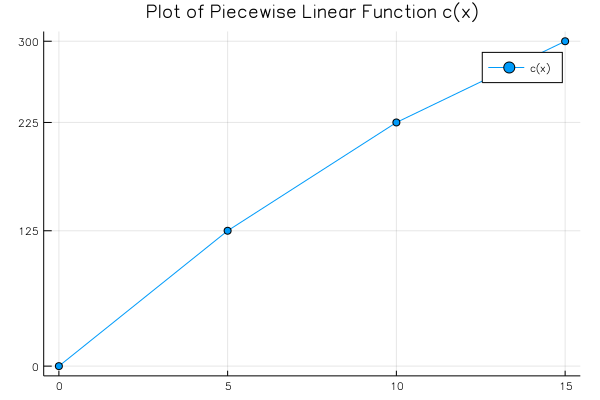
\includegraphics[scale = 0.2]{pwl-plot.png}
\end{center}
We will use integer programming to describe this function.  We will fix $x = a$ and then the integer program will set the value $y$ to $c(a)$.
\begin{align*}
\min\quad & 0\\
\text{Subject to} \quad & x - 5 z_{2} - 10 z_{3} - 15 z_{4} = 0\\
 & y - 125 z_{2} - 225 z_{3} - 300 z_{4} = 0\\
 & z_{1} + z_{2} + z_{3} + z_{4} = 1\\
 & SOS2: \{z_1, z_2, z_3, z_4\}\\
 & 0 \leq z_{i} \leq 1 \quad\forall i \in \{1,2,3,4\}\\
 & x = a\\
\end{align*}

\end{examplewithcode}

\begin{examplewithcode}{Piecewise Linear Function Application}{code:pwl-application}
\label{example:pwl-application}
Consider the following optimization problem where the objective function includes the term $c(x)$, where $c(x)$ is the piecewise linear function described in \nameref{example:pwl}:
$$
\begin{array}{cc}
\max & z = 12x_{11} + 12x_{21} + 14x_{12} + 14x_{22} - c(x)\\
\text{s.t.} & x_{11} + x_{12} \leq x + 5\\
& x_{21} + x_{22} \leq 10\\
& 0.5 x_{11} - 0.5x_{21} \geq 0\\
& 0.4 x_{12} - 0.6 x_{22} \geq 0\\
& x_{ij} \geq 0\\
& 0 \leq x \leq 15
\end{array}
$$

Given the piecewise linear, we can model the whole problem explicitly as a mixed-integer linear program.

 \begin{align*}
 \max\quad & 12 X_{1,1} + 12 X_{2,1} + 14 X_{1,2} + 14 X_{2,2} - y\\
\text{Subject to} \quad & x - 5 z_{2} - 10 z_{3} - 15 z_{4} = 0\\
 & y - 125 z_{2} - 225 z_{3} - 300 z_{4} = 0\\
 & z_{1} + z_{2} + z_{3} + z_{4} = 1\\
 & X_{1,1} + X_{1,2} - x \leq 5\\
 & X_{2,1} + X_{2,2} \leq 10\\
 & 0.5 X_{1,1} - 0.5 X_{2,1} \geq 0\\
 & 0.4 X_{1,2} - 0.6 X_{2,2} \geq 0\\
 & SOS2: \{z_1, z_2, z_3, z_4\}\\
 & X_{i,j} \geq 0 \quad\forall i \in \{1,2\}, j \in \{1,2\}\\
 & 0 \leq z_{i} \leq 1 \quad\forall i \in \{1,2,3,4\}\\
 & 0 \leq x \leq 15\\
 & y\\
\end{align*}

\end{examplewithcode}


\subsection{Maximizing a minimum}
When the constraints could be general, we will write $x \in X$ to define general constraints.  For instance, we could have $X = \{ x \in \R^n : Ax \leq b\}$ of $X  = \{ x \in \R^n : Ax \leq b, x \in \Z^n\}$ or many other possibilities.  


Consider the problem 

\begin{align*}
\max   \quad & \min \{x_1, \dots, x_n\}\\
\text{ such that } \quad &  x \in X
\end{align*}
Having the minimum on the inside is inconvenient.  To remove this, we just define a new variable $y$ and enforce that $y \leq x_i$ and then we maximize $y$.  Since we are maximizing $y$, it will take the value of the smallest $x_i$.  Thus, we can recast the problem as

\begin{align*}
\max\quad    & y\\
\text{ such that } \quad  & y \leq x_i \ \text{ for }\  i=1, \dots, n \\
&  x \in X
\end{align*}


\subsection{Relaxing (nonlinear) equality constraints}

There are a number of scenarios where the constraints can be relaxed without sacrificing optimal solutions to your problem.   In a similar vein of the maximizing a minimum, if because of the objective we know that certain constraints will be tight at optimal solutions, we can relax the equality to an inequality.   For example, 
\begin{align*}
\max   \quad &x_1 + x_2 +  \dots + x_n\\
\text{ such that } \quad &  x_i = y_i^2 + z_i^2 \text{ for } i=1, \dots, n
\end{align*}






\section{Notes from AIMMS modeling book.}
\begin{itemize}

\item \href{http://inside.mines.edu/~anewman/MIP_practice120212.pdf}{AIMMS - Practical guidelines for solving difficult MILPs}

\item \href{https://download.aimms.com/aimms/download/manuals/AIMMS3OM_LinearProgrammingTricks.pdf}{AIMMS - Linear Programming Tricks}


\item  \href{https://download.aimms.com/aimms/download/manuals/AIMMS3OM_FormulatingOptimizationModels.pdf}{AIMMS - Formulating Optimization Models}


\item \href{https://pdfs.semanticscholar.org/b01f/ad44c20c372fdda95cbfb980c0d37302de07.pdf}{AIMMS - Practical guidelines for solving difficult linear programs}
\end{itemize}
\subsection{Further Topics}
\begin{itemize}
\item \href{https://or.stackexchange.com/questions/1319/best-model-for-precedence-constraints-within-scheduling-problem}{Precedence Constraints}
\end{itemize}

\end{document}
